% Slide 64: Online Lectures
\begin{frame}{سخنرانی‌ها و منابع برخط}{\lr{Online Lectures}}
  \begin{columns}[T]
    \begin{column}{0.54\textwidth}
      \begin{itemize}
        \setlength{\itemsep}{6pt}
        \item مطالب تکمیلی این هفته پیرامون \textbf{خوشه‌بندی سلسله‌مراتبی \lr{(Hierarchical Clustering)}} ارائه شده است.
        \item ویدیوها و اسلایدهای آموزشی برخط مکمل مباحث کلاس بوده و برای تمرین‌های عملی و امتحانات پایانی \textbf{بسیار حائز اهمیت} می‌باشند.
      \end{itemize}
    \end{column}
    \begin{column}{0.44\textwidth}
      \begin{center}
        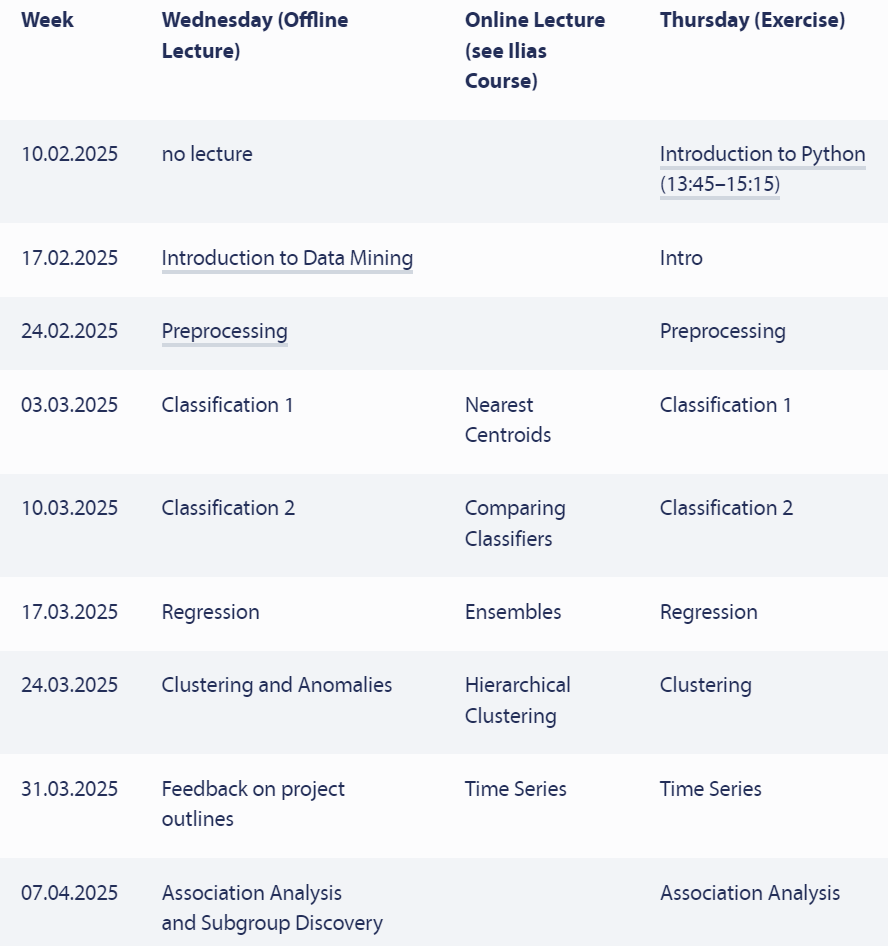
\includegraphics[width=\textwidth,height=4.6cm,keepaspectratio]{images/slide64_online_lecture.png}
      \end{center}
    \end{column}
  \end{columns}
\end{frame}

% Slide 65: Questions?
\begin{frame}{پرسش و پاسخ}{\lr{Questions?}}
  \begin{center}
    \vspace*{0.4cm}
    
\includegraphics[height=4.2cm,keepaspectratio]{images/slide65_questions.png}\\[0.4cm]
    {\fontsize{14}{18}\selectfont\color{mannheimblue}\textbf{آیا پرسشی در مورد این فصل دارید؟}}\\[0.2cm]
    {\fontsize{9}{12}\selectfont\color{subgray}خوشه‌بندی و تشخیص ناهنجاری در داده‌کاوی}
  \end{center}
\end{frame}

% Slide 66: Literature
\begin{frame}{منابع و مراجع مطالعاتی}{\lr{Literature for this Slideset}}
  \begin{columns}[T]
    \begin{column}{0.62\textwidth}
      {\fontsize{8.5}{11.5}\selectfont
      \textbf{کتاب مرجع اصلی:}
      \begin{itemize}
        \setlength{\itemsep}{3pt}
        \item \lr{Pang-Ning Tan, Michael Steinbach, Anuj Karpatne, Vipin Kumar:} \\
        \textbf{\lr{Introduction to Data Mining}}, \lr{2nd Edition, Pearson.}
      \end{itemize}
      \vspace{0.2cm}
      \textbf{فصول مرتبط از کتاب:}
      \begin{itemize}
        \setlength{\itemsep}{2pt}
        \item \textbf{فصل ۵: تحلیل خوشه \lr{(Chapter 5: Cluster Analysis)}}
        \begin{itemize}
          \item بخش ۵.۲: الگوریتم کا-میانگین \lr{(K-Means)}
          \item بخش ۵.۳: خوشه‌بندی سلسله‌مراتبی تراکمی \lr{(Agglomerative Hierarchical)}
          \item بخش ۵.۴: الگوریتم \lr{DBSCAN}
        \end{itemize}
        \item \textbf{فصل ۲: بخش ۲.۴:} معیارهای شباهت و عدم‌شباهت \lr{(Similarity \& Dissimilarity Measures)}
      \end{itemize}
      }
    \end{column}
    \begin{column}{0.35\textwidth}
      \begin{center}
        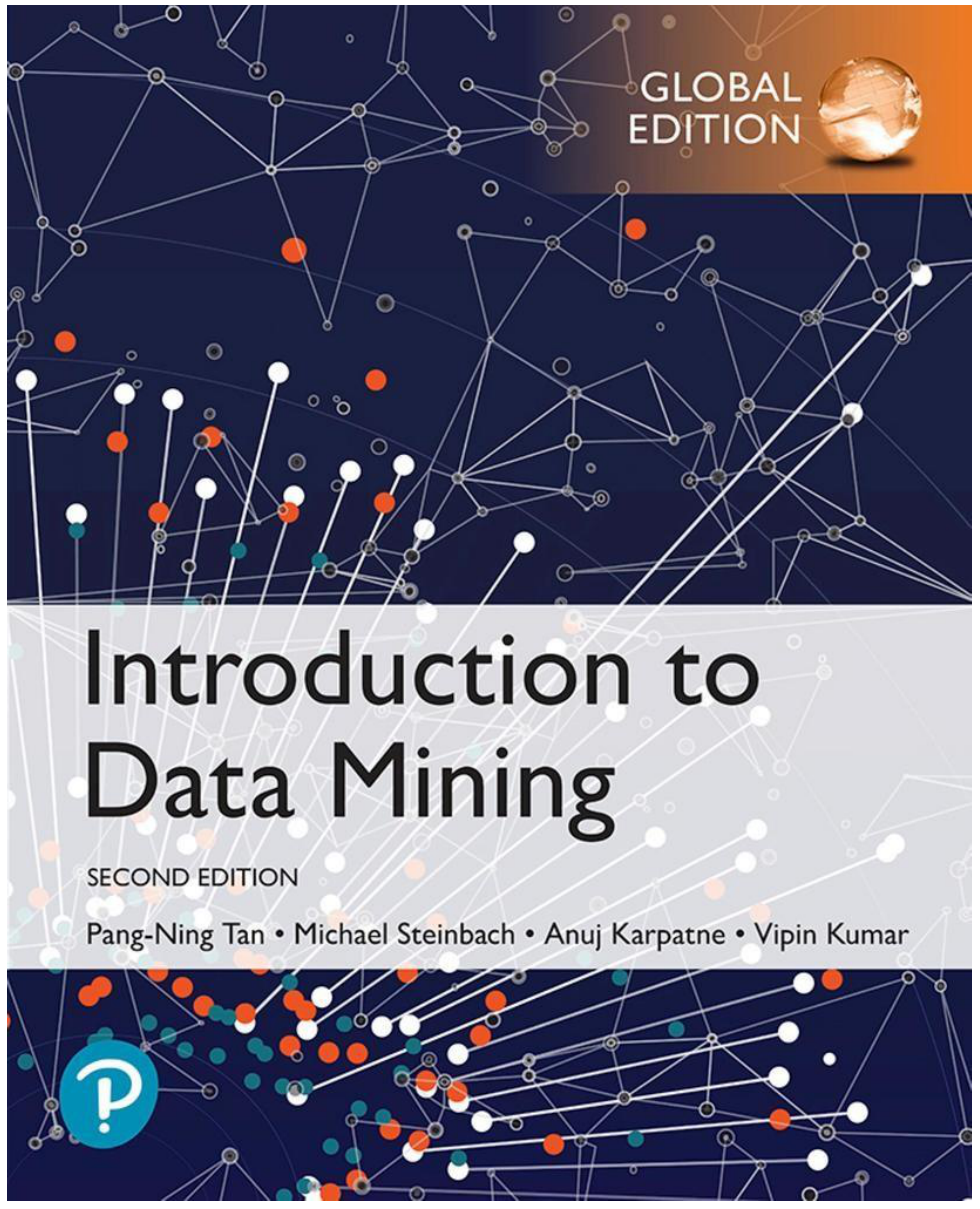
\includegraphics[width=\textwidth,height=4.8cm,keepaspectratio]{images/slide66_book_covers.png}
      \end{center}
    \end{column}
  \end{columns}
\end{frame}
